\documentclass[12pt,epsf,psfig,graphicx]{article}             

% \documentstyle[bookman,epsf]{article}             
\textwidth = 6.5in
\textheight = 9.05in
\topmargin 0.0in
\oddsidemargin 0.0in
\evensidemargin 0.0in

\usepackage[T1]{fontenc}
\usepackage{mathptmx}
\usepackage{graphicx}

% set it so that subsubsections have numbers and they
% are displayed in the TOC (maybe hard to read, might want to disable)

\setcounter{secnumdepth}{3}
\setcounter{tocdepth}{3}

% define widow protection 
        
\def\widow#1{\vskip #1\vbadness10000\penalty-200\vskip-#1}

% define a little section heading that doesn't go with any number

\def\littlesection#1{
\widow{2cm}
\vskip 0.5cm
\noindent{\bf #1}
\vskip 0.1cm
\noindent
}

% A paraphrase mode that makes it easy to see the stuff that shouldn't
% stay in for the final proposal

\newdimen\tmpdim
\long\def\paraphrase#1{{\parskip=0pt\hfil\break
\tmpdim=\hsize\advance\tmpdim by -15pt\noindent%
\hbox to \hsize
{\vrule\hskip 3pt\vrule\hfil\hbox to \tmpdim{\vbox{\hsize=\tmpdim
\def\par{\leavevmode\endgraf}
\obeyspaces \obeylines 
\let\par=\endgraf
\bf #1}}}}}

\renewcommand{\baselinestretch}{1.2}    % must go before the begin of doc
\newtheorem{principle}{Principle}
\newtheorem{definition}{Definition}
% go with the way that CC sets the margins

\begin{document}

% handle widows appropriately
\def\widow#1{\vskip #1\vbadness10000\penalty-200\vskip-#1}

\begin{center}

CS290: Principles of Software Development \\
Examination Two \\

\end{center}

\noindent Answer the five questions that are listed on the following pages.  You must provide answers to these questions
on a separate sheet of paper.  Please develop responses that clearly express your ideas in the most succinct manner
possible.  You are not permitted to complete this examination in conjunction with any of your classmates.  Furthermore,
you cannot consult any outside references during this examination.  If you have questions concerning the following
problems, then please visit my office during the examination period.  If you leave the classroom to take the exam, then
you are responsible for checking the white board for status updates.

% \noindent Answer the five questions that are listed below.  You must provide answers to these questions on a separate
% sheet of paper.  Please develop responses that clearly express your ideas in the most succinct manner possible.  You are
% not permitted to complete this examination in conjunction with any of your classmates.  Furthermore, you cannot consult
% any outside references during this examination.  If you have questions concerning the problems that are listed below,
% then please visit my office during the examination period.  If you leave the classroom to take the exam, then you are
% responsible for checking the white board for status updates.
% 
\begin{enumerate}

\item ({\bf 10 Points}) Requirements elicitation and analysis is an important part of the overall software life cycle.
	Answer the following questions about software requirements.

\begin{enumerate}

	\item ({\bf 2 Points}) What is a software requirement? Why is it important to define the requirements of a software
		application before starting to implement it?

	\item ({\bf 4 Points}) Please define and give at least one example of each type of requirement.

		\begin{enumerate}
			\item Functional requirement
			\item Non-functional requirement
			\item Design constraint
			\item Process constraint
		\end{enumerate}

	\item ({\bf 4 Points}) There are at least eight ``requirements'' for software requirements.  Please name and define
		four of the eight requirements; state the importance of each of these.


% What is a software requirement?

% \item ({\bf 6 Points}) Sommerville argues that there are six
%   requirements to which all requirements should adhere.  What are
%   these six requirements?
% 

% \item ({\bf 3 Points}) Software engineers commonly organize
%   requirements into the following three categories: {\em functional},
%   {\em non-functional}, and {\em domain}.  Please provide a definition
%   and an example of these three types of requirements.
% 
\end{enumerate}

\newpage

\begin{figure}[t]
	\centering
	\begin{tabular}{c c}
		\begin{minipage}{3.4in} 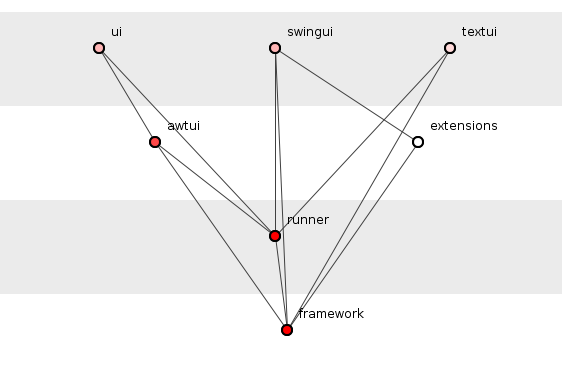
\includegraphics[width=3in]{37.png} \vspace*{-.2in} \begin{center}(a)\end{center} \end{minipage} & 
		\begin{minipage}{3.4in} 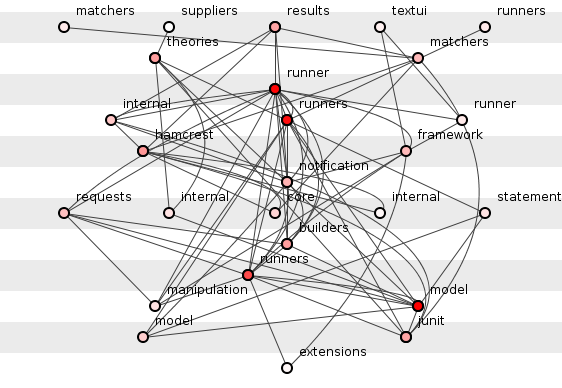
\includegraphics[width=3in]{45.png} \vspace*{-.2in} \begin{center}(b)\end{center} \end{minipage}
 	\end{tabular}
	\caption{The Evolving Architecture of the JUnit Test Automation Framework.}
	\label{fig:junit}
\end{figure}

\item ({\bf 10 Points}) An engineer must be able to capture and use the requirements for a system.  Answer the following
	questions about requirements elicitation and software architecture.

\begin{enumerate}

\item ({\bf 2 Points}) Francis Bacon said that ``truth emerges more
  readily from error than confusion.''  What does this quote mean?
  How does it apply to the task of requirements elicitation and
  analysis?

% \item ({\bf 4 Points}) The process for capturing the requirements of a
%   software system normally includes four distinct phases.  Draw a
%   diagram that shows each of these phases and indicates how a software
%   engineer can proceed through them.  In your diagram, a square or a
%   rectangle should denote a phase and a directed edge should show a
%   possible way to follow from one phase to the next.
% 

% \item ({\bf 2 Points}) Hamlet and Maybee argue that requirements
%   should be {\em non-prescriptive}.  What does it mean if a
%   requirement has this characteristic?  After defining this term,
%   please give an example of a non-prescriptive requirement.
% 
\end{enumerate}

\newpage

\item ({\bf 10 Points}) Research in software architectures has
  flourished in recent years.  Answer the following questions about
  software architectures by providing a response for each part.

\begin{enumerate}

% \item ({\bf 2 Points}) Define the term software architecture.  Discuss
%   some of the advantages to explicitly designing and documenting a
%   software architecture.
% 
\item ({\bf 3 Points}) The {\em shared} repository (or {\em tuple
  space} or {\em blackboard}) model is one example of a software
  architecture.  Please draw a diagram that explains how this
  architecture works.  What is one strength and one weakness of this
  architecture?

\item ({\bf 3 Points}) The pipe and filter is another example of a
  software architecture.  In the context of this architecture, what is
  the meaning of the terms {\em pipe} and {\em filter}?  Your response
  to this question should also furnish an example of a pipe and filter
  architecture in the context of the GNU/Linux command line.

\item ({\bf 2 Points}) One benefit of the pipe and filter architecture
  is that it supports the easy analysis of throughput and response
  time.  Draw two graphs that explain the relationship between {\em
    throughput} and {\em response time} and the {\em length} of the
  pipe and filter chain.  The first graph should have the label
  ``throughput'' on the vertical axis and ``length of the pipe and
  filter chain'' on the horizontal while the second should have
  ``response time'' on the vertical and ``length of the pipe and
  filter chain'' on the horizontal.

\end{enumerate}

\newpage

\item ({\bf 10 Points}) It is essential for a software system to have
  a design that is easy to understand and implement.  Answer the
  following questions about the software design process.

\begin{enumerate}

\item ({\bf 2 Points}) Define the term {\em model} and clearly state
  the fundamental reason for the creation of models during the
  development of software.

\item ({\bf 4 Points}) The unified modeling language supports the
  creation of {\em class diagrams} that can illustrate inheritance
  hierarchies.  What is an {\em inheritance hierarchy}?  Why is it
  useful to create inheritance hierarchies in object-oriented
  programs?  Your response to this question should also provide an
  example of a class diagram.

\item ({\bf 4 Points}) The unified modeling language provides
  diagrams that visualize both {\em static} and {\em dynamic} views of
  a software system.  After explaining the terms static and dynamic
  view, your response to this question should discuss the similarities
  and differences between these two types of views.

\end{enumerate}

\newpage

\item ({\bf 10 Points}) When it comes to developing high quality
  software applications, it is important to properly complete all of
  the phases of the software lifecycle.  Answer the following
  questions about the lifecycle of engineering software.

\begin{enumerate}

\item ({\bf 4 Points}) Suppose that you are part of a development team
  that is responsible for implementing a compiler for the Java
  programming language.  The manager of your team asks you to fully
  implement {\em array-bounds checking} in your compiler.  After
  defining what this term means, explain whether or not this
  requirement is {\em feasible}.

\item ({\bf 2 Points}) After conducting an empirical investigation of
  software errors, Basili and Perricone draw the following conclusion:
  ``48 percent of faults observed in a medium-scale software project
  were attributed to incorrect or misinterpreted functional
  specifications or requirements.''  In your opinion, why is this the
  case?

% \item ({\bf 4 Points}) It is important to develop ways to rate
%   the quality of a requirements document since the individual
%   requirements are used by the designers, implementers, and
%   testers throughout the remainder of the lifecycle.  Pfleeger
%   and Atlee outline the following scale for evaluating a
%   requirement:
% 
% \renewcommand{\labelitemi}{$-$}
% 
%           \begin{itemize}
% 
%           \item 1 - You (the designer) understand this requirement
%             completely, you have designed from similar requirements in
%             the past, and you should have no trouble developing a
%             design from this requirement.
% 
%           \item 2 - There are elements of this requirement that are
%             new to you, but they are not radically different from
%             requirements that you have successfully designed from in
%             the past.
% 
%           \item 3 - There are elements of this requirements that are
%             very different from requirements that you have designed
%             from in the past, but you understand the requirement and
%             you think that you can develop a good design from it.
% 
%           \item 4 - There are parts of this requirement that you do
%             not understand, and you are not sure that you can develop
%             a good design.
% 
%           \item 5 - You do not understand this requirement at all, and
%             you cannot develop a design for it.
% 
%           \end{itemize}
% 
%           Using this rating scheme, it is possible to determine
%           whether or not a software development team should start to
%           design and implement the system.  As part of your response
%           to this question, please draw two {\em histograms} where the
%           vertical axis is the {\em number} of requirements in each of
%           the above categories and the horizontal axis gives the {\em
%             categories} in numerically increasing order (i.e., 1 to
%           5).  One of the histograms must represent a system that is
%           ready to leave the requirements elicitation and analysis
%           phase and the other should reveal that it is not advisable
%           to start the architecture and design phase.  Your response
%           should clearly explain why you created the histograms in
%           this way.
% 
\end{enumerate}

\end{enumerate}

\end{document}



